\section{Methods}

\subsection{Participants and Task}
Twenty-four adults (mean age 27.31 years) performed a numerical
change-detection task using an oddball paradigm with dot-array stimuli
representing quantities 1-6. EEG was recorded continuously at 250 Hz
from a 128-channel EGI HydroCel Geodesic Sensor Net.
Each trial consisted of 3-5 ``prime'' images of the same numerosity
(250 ms each, jittered ISI of 750-1250 ms), followed by a target
image. On change trials, the target differed from the prime and
participants pressed a button to indicate they detected a change.
Each change trial is defined by its prime-target pair. For example,
a trial with prime 4 and target 2 is coded as condition ``42.''
Prime and target always differ by at most 3 items within the 1-6
range, yielding 24 unique prime-target conditions
(Figure~\ref{fig:task-design}). We analyzed all change trials
(both correct and incorrect responses), resulting in 216 usable
epochs per participant (9 trials per condition per participant).

\begin{figure}[!t]
  \centering
  \begin{minipage}[t]{\columnwidth}
    \centering
    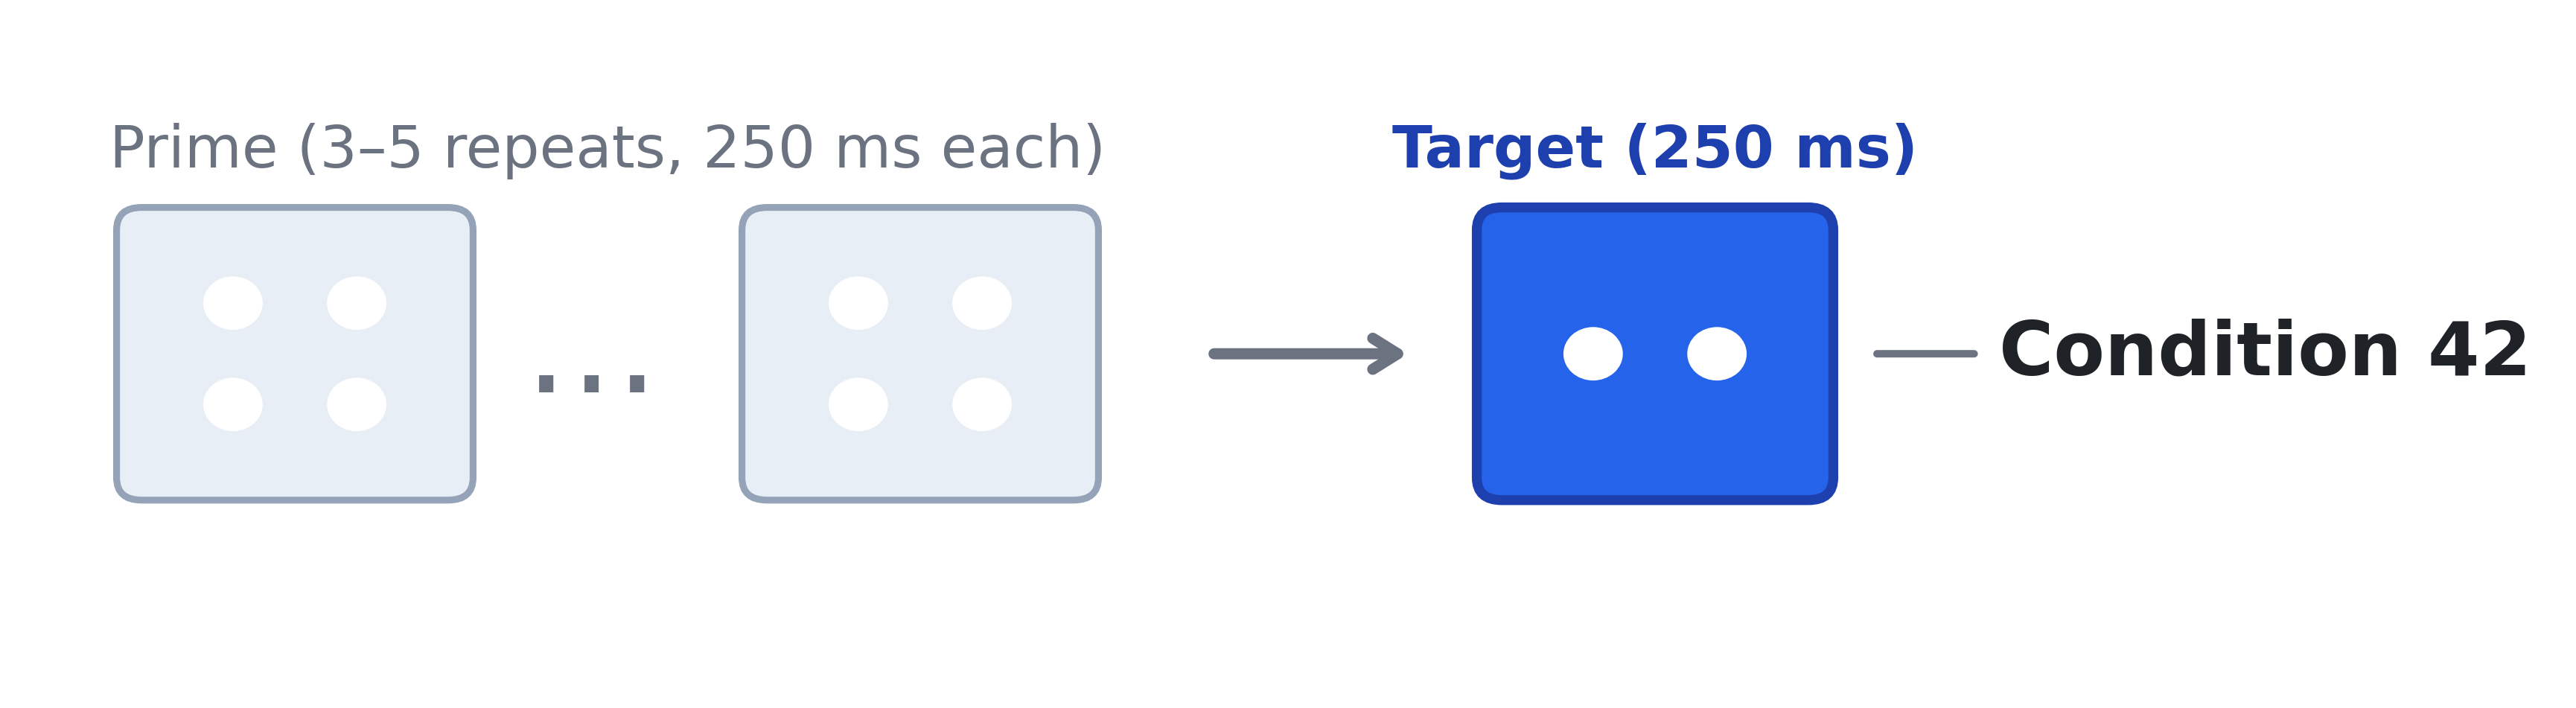
\includegraphics[width=0.85\columnwidth]{media/trial_structure.png}
    \vspace{-1mm}
    \subcaption{Single-trial structure. Three to five identical prime
    images precede a target that differs in numerosity. Condition codes
    denote the prime-target pair (e.g., ``42'' = prime 4, target 2).}
    \label{fig:trial-structure}
  \end{minipage}

  \vspace{4pt}

  \begin{minipage}[t]{\columnwidth}
    \centering
    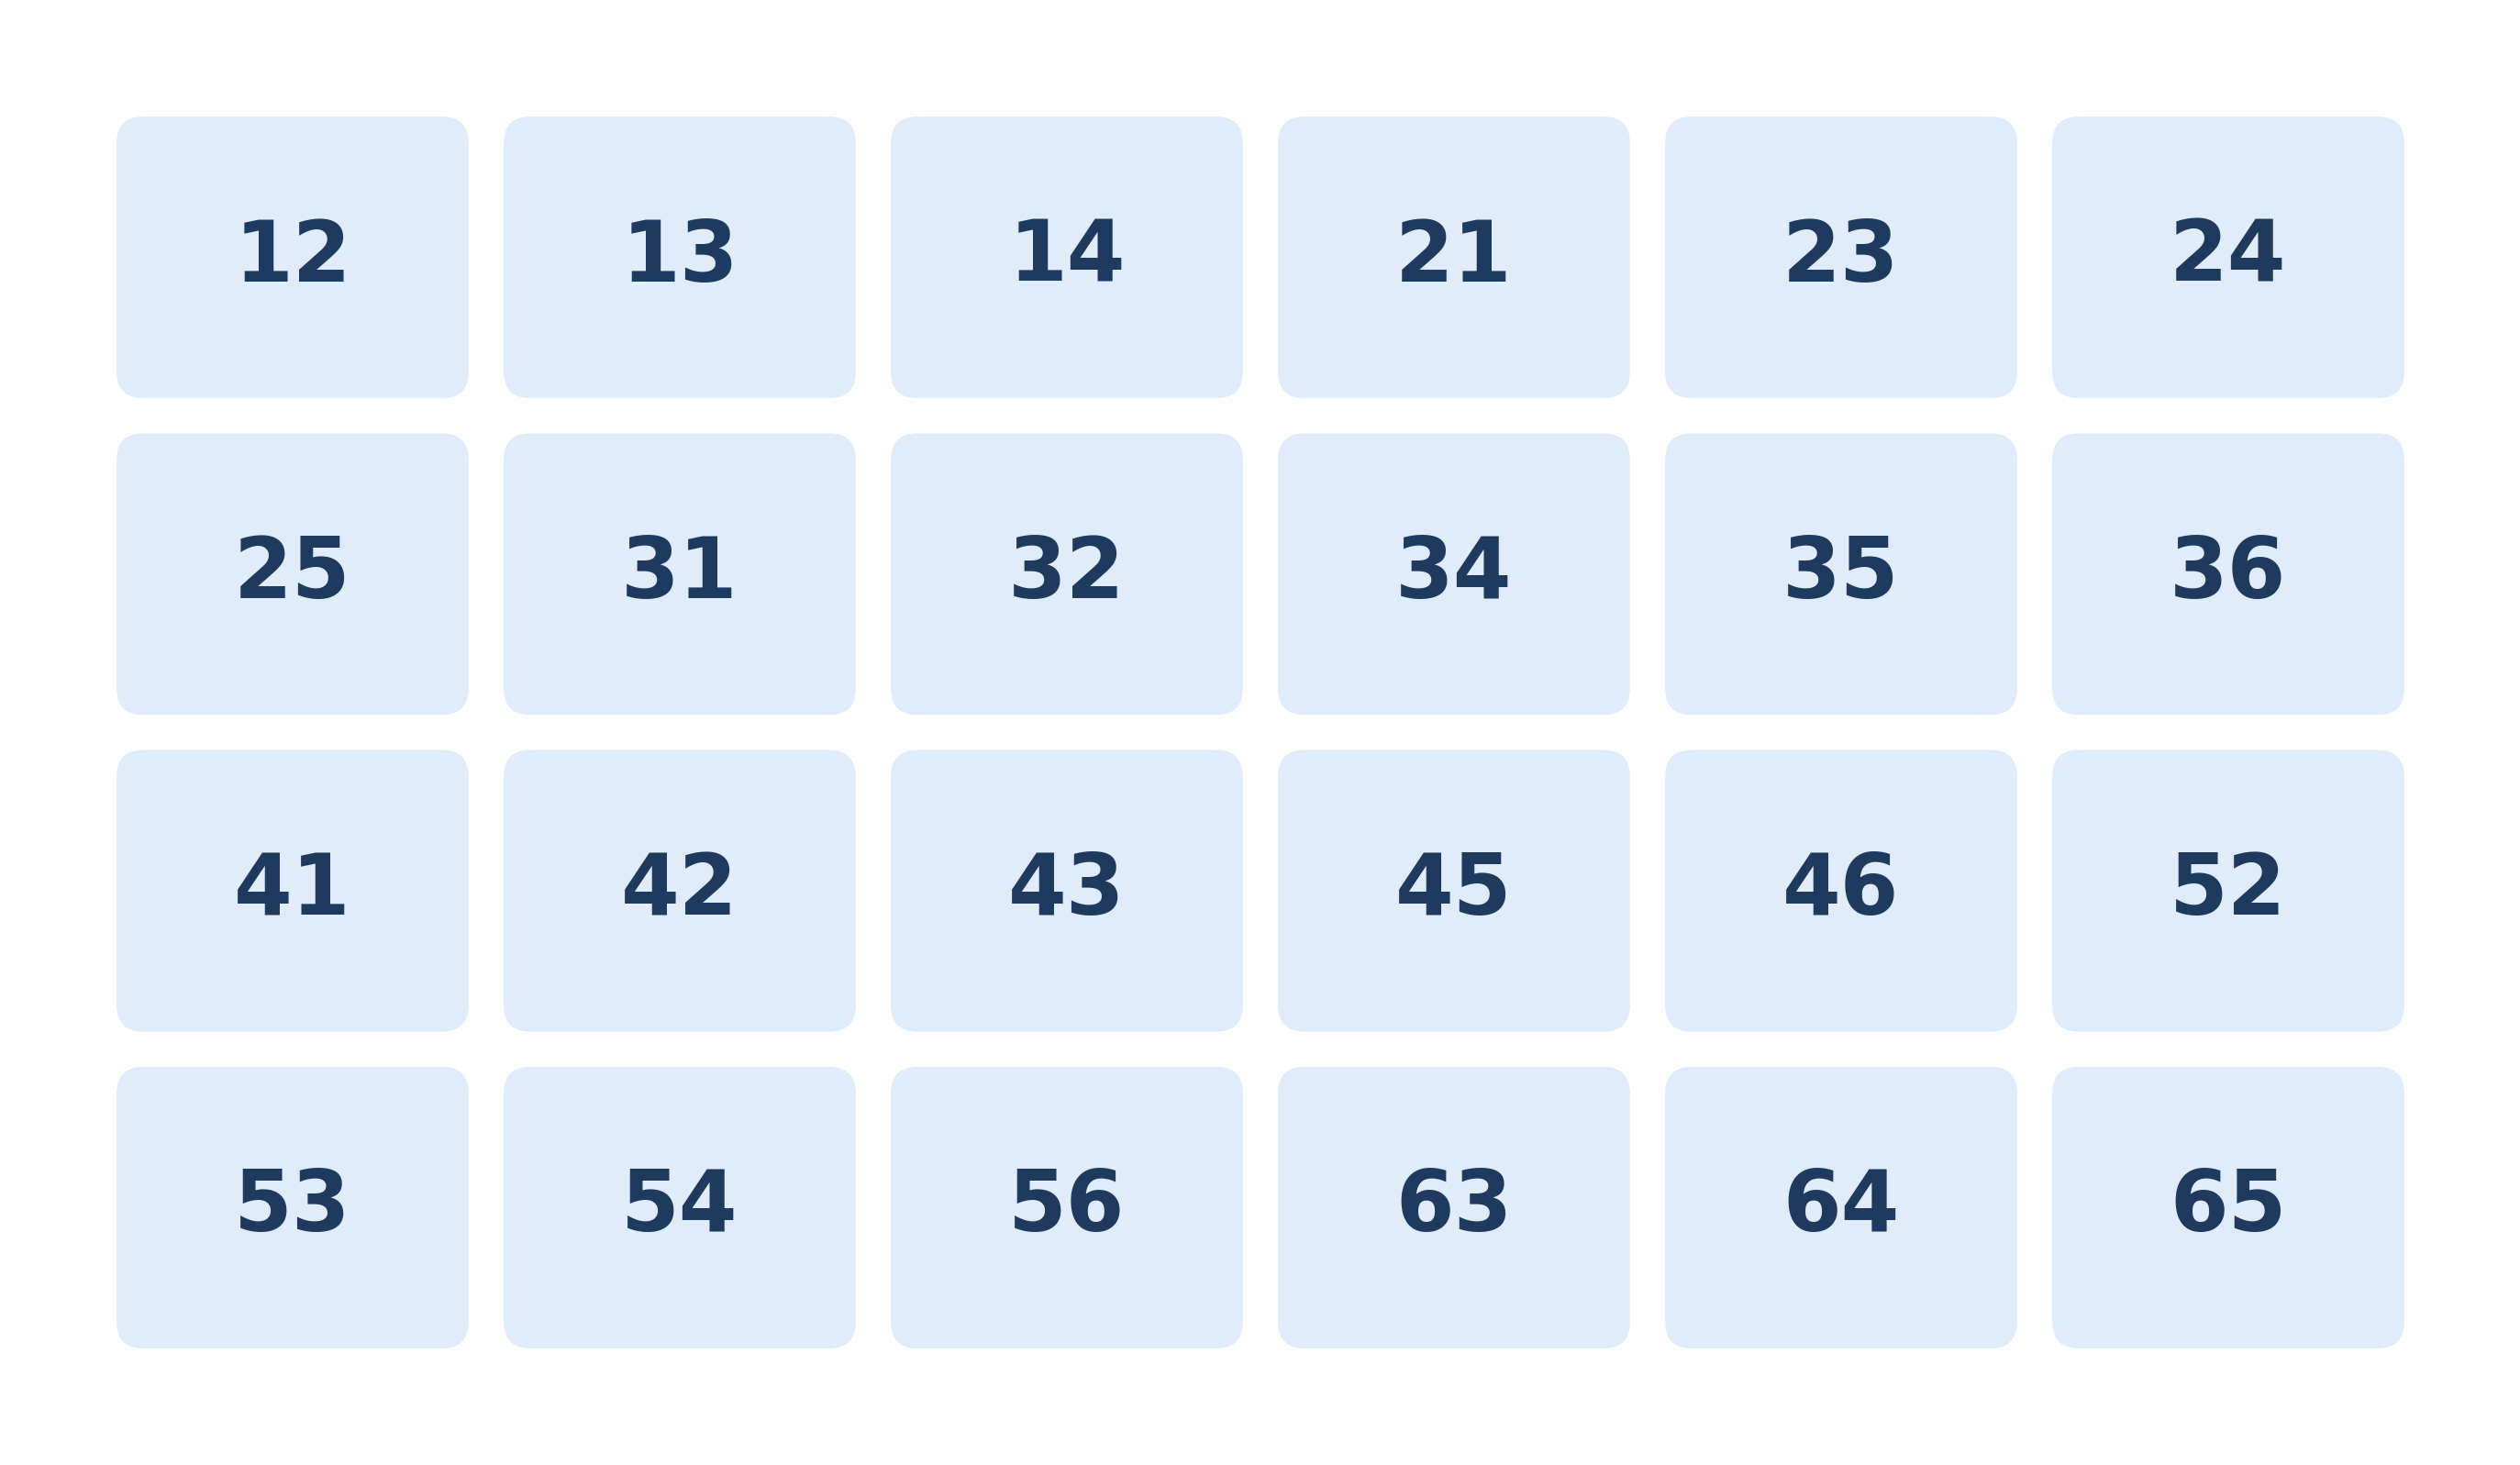
\includegraphics[width=0.75\columnwidth]{media/conditions-24.png}
    \vspace{-1mm}
    \subcaption{All 24 prime-target change conditions used in this
    study. Prime and target differ by 1-3 items within the 1-6 range.}
    \label{fig:condition-matrix}
  \end{minipage}

  \vspace{4pt}

  \begin{minipage}[t]{\columnwidth}
    \centering
    
\includegraphics[width=0.70\columnwidth]{media/conditions-6.png}
    \vspace{-1mm}
    \subcaption{Whole-epoch target numerosities (1-6), obtained by
    collapsing across prime identity in (b).}
    \label{fig:condition-6}
  \end{minipage}
  \caption{Task design.}
  \label{fig:task-design}
\end{figure}


\subsection{Preprocessing}
EEG data were preprocessed using the Harvard Automated Processing Pipeline
for Electroencephalography \citep[HAPPE v4.1.0;][]{GabardDurnam2018HAPPE}.
Preprocessing included a 1.5-35 Hz bandpass filter and 60 Hz line-noise
removal (CleanLine). HAPPE identified and interpolated bad
channels and applied wavelet-based artifact correction (soft
thresholding).
Each epoch was baseline-corrected using the prestimulus interval
(-200 to 0 ms).

\subsection{Representational Similarity Analysis}
We used Representational Similarity Analysis (RSA) to compare neural
and theoretical dissimilarity structures \citep{Kriegeskorte2008}.
For each pair of conditions, we trained a classifier to discriminate
the two conditions and used the resulting binary decoding accuracies to construct
a neural representational dissimilarity matrix (RDM). We then correlated these neural RDMs with
theoretical model RDMs encoding competing hypotheses about numerosity
representation.

We used Linear Discriminant Analysis (LDA) with Ledoit-Wolf
regularization (scikit-learn, \citealp{Pedregosa2011}) for binary
numerosity classification. To prevent data leakage
\citep{KapoorNarayanan2023Leakage}, we used subject-wise GroupKFold
cross-validation (6 folds), so that no subject appeared in both
training and test sets within a fold. Cluster-based permutation tests
used MNE-Python \citep{Gramfort2013}.

\subsection{Theoretical Model RDMs}
The following theoretical RDMs encode competing hypotheses about the
representational structure of numerosity and serve as predictions
for whole-epoch and temporal analyses
(Figures~\ref{fig:static-model-rdms} and~\ref{fig:temporal-change24-model-rdms}).
\begin{itemize}
  \item \textbf{Target PI}: A family of models encoding the target's
    system membership. Numerosities at
    or below a boundary $B$ are assigned to PI, and those above $B$ to
    ANS. Within PI, dissimilarity is a fixed constant (categorical).
    Within ANS, dissimilarity follows $|\log(a/b)|$. Cross-system
    pairs receive an elevated baseline plus log-ratio scaling:
    $d = c + |\log(a/b)|$, where $c$ is a boundary constant. We
    tested two boundary locations ($B = 4$ and $B = 3$) crossed with
    two numerosity ranges (1-6 and 2-6), yielding four variants:
    Target PI(1-4), Target PI(1-3), Target PI(2-4), and Target
    PI(2-3). The no-1 variants exclude numerosity~1 from both prime
    and target during training and evaluation.
  \item \textbf{ANS}: A graded distance model assuming a single
    continuous magnitude code with no categorical boundary.
    Dissimilarity scales with numerical ratio following Weber's law,
    $d(i,j) = |\log(a/b)|$.
  \item \textbf{Pixel}: A visual control model, included because
    dot-array stimuli covary with low-level properties such as total
    area and density.
    $d(i,j) = |\text{area}_i - \text{area}_j|$,
    the absolute difference in total white-pixel area between the two
    stimulus images.
  \item \textbf{RT}: A behavioral-difficulty control model.
    $d(i,j) = |\overline{\text{RT}}_i -
    \overline{\text{RT}}_j|$, the absolute difference in grand-mean
    reaction time between conditions. RTs were computed from correct
    trials only, winsorized at the 2.5th and 97.5th percentiles within
    each subject and condition, then averaged across subjects.
\end{itemize}

\begin{figure*}[!t]
  \centering
  \begin{minipage}{\textwidth}
    \centering
    \textbf{(a)} Target-only analysis (numerosities 1-6)\par\smallskip
    \includegraphics[width=\textwidth]{../results/analysis-lda/static-change6/static_change6_all/figures-pairwise/temporal_model_rdms_all_compact_row-static_change6_all-pairwise.png}
  \end{minipage}
  \vspace{4pt}
  \begin{minipage}{\textwidth}
    \centering
    \textbf{(b)} Target-only no-1 analysis (numerosities 2-6)\par\smallskip
    \includegraphics[width=\textwidth]{../results/analysis-lda/static-change5/static_change5_all/figures-pairwise/temporal_model_rdms_all_compact_row-static_change5_all-pairwise.png}
  \end{minipage}
  \caption{Brain and model RDMs (0-700 ms). Brain RDMs show mean
  balanced accuracy (\%) across subjects. Model RDMs show predicted
  dissimilarity for each theoretical model. The RT model shows absolute
  differences in grand-mean reaction time. The Pixel model shows
  absolute differences in white-pixel area. In this stimulus set, total
  area is similar within numerosities 1-3 and within 4-6 but drops
  sharply between 3 and 4, so the Pixel model's largest discontinuity
  falls at 3-4. (a)~Target numerosities 1-6. Pairs involving
  numerosity~1 show the highest discriminability, giving the brain RDM
  an ANS-like gradient dominated by distance from~1
  (Table~\ref{tab:static-model-comparison}). In the boundary region,
  pairs 4-5 and 4-6 show slightly higher discriminability than pairs 2-4
  and 3-4, consistent with a boundary at 4-5 rather than 3-4.
  (b)~Target numerosities 2-6 (numerosity~1 excluded from both prime and
  target during training and evaluation). With numerosity~1 removed, the
  boundary structure becomes clearer. Pairs crossing the 4-5 boundary
  (4-5, 4-6) show higher discriminability than pairs within the PI range
  (2-4, 3-4), matching the Target PI(2-4) prediction
  (Table~\ref{tab:static-model-comparison}). The Pixel model predicts
  the opposite pattern, with highest dissimilarity across the 3-4
  boundary, and does not reach significance
  (Table~\ref{tab:static-model-comparison}).}
  \label{fig:static-model-rdms}
\end{figure*}


We used a two-part analysis strategy to balance sensitivity to stable
representational structure and temporal resolution. The whole-epoch
analysis tests whether a target numerosity structure is present when
evidence is aggregated across the post-stimulus interval. The temporal
analysis tests how numerosity-related structure evolves over time using
time-resolved neural RDMs that preserve prime-target condition
identity.

\subsection{Whole-Epoch Target RSA}
The whole-epoch analysis collapses across prime identity, retaining
only the target numerosity (Figure~\ref{fig:condition-6}). LDA classifiers discriminated between
target numerosities over a 0-700 ms post-stimulus epoch (no sliding
window), producing a single RDM per subject. This analysis
has two variants: the target-only analysis (numerosities 1-6) and the
target-only no-1 analysis (numerosities 2-6), which excludes
numerosity~1 from both prime and target during classifier training
and evaluation. This no-1 variant isolates boundary structure in the
2-6 range by separating it from effects specific to numerosity~1.

\subsection{Temporal RSA}
Sliding-window RSA (50 ms window, 20 ms stride) used window
centers from $-100$ to 700 ms relative to target onset (first
window: $-125$ to $-75$ ms, centered at $-100$ ms; subsequent windows
advanced by 20 ms), using the full 24-condition prime-target structure
(Figure~\ref{fig:condition-matrix}). Each time window produces a
24 $\times$ 24 RDM that preserves the identity of both prime and
target. For the no-1 control, pairs containing numerosity~1 are
excluded from the existing RDM,
reducing the matrix to 18 $\times$ 18.

\subsection{Statistics}
Spearman correlation ($\rho$) quantified model-brain similarity, and
multidimensional scaling (MDS) visualized representational geometry
\citep{Kriegeskorte2008}. To contextualize model-fit magnitudes, we
computed a lower-bound noise ceiling using leave-one-subject-out
cross-validation: for each subject, we correlated that subject's neural
RDM with the mean RDM of all remaining subjects, then averaged across
subjects. For temporal analyses, this was computed at each time window.

For the whole-epoch analysis, one-sample $t$-tests (Holm-corrected
across models) assessed significance of Fisher-$z$-transformed
per-subject model correlations. Boundary contrasts compared Target
PI(x-4) versus Target PI(x-3) using paired $t$-tests on Fisher-$z$
differences (two-sided, Cohen's $d_z$).

For the temporal analysis, cluster-based permutation tests (5,000
permutations, $\alpha = 0.05$) identified sustained periods of
significant model-brain correlation. Cluster-forming thresholds used
the $t$-critical value with $\text{df} = N - 1$ (one-sided for
model-fit tests), with a minimum cluster size of 2 consecutive
windows. Individual decoding accuracy was tested against chance using
the same one-sided cluster-based permutation framework.

Model comparisons applied the same framework to
Fisher-$z$-transformed Spearman correlation differences at each time
window (10,000 permutations, two-sided, $\alpha = 0.05$), including
boundary-location tests (4-5 vs.\ 3-4). All analyses were repeated
with and without numerosity~1.
